\documentclass[11pt,onecolumn,a4paper]{report}

\usepackage{icb}
\usepackage{times}
\usepackage{epsfig}
\usepackage{epstopdf}
\usepackage{graphicx}
\usepackage{amsmath}
\usepackage{amssymb}
\usepackage{listings}
\usepackage{url}
\usepackage[english,german]{babel}

% Include other packages here, before hyperref.

% If you comment hyperref and then uncomment it, you should delete
% egpaper.aux before re-running latex.  (Or just hit 'q' on the first latex
% run, let it finish, and you should be clear).
%\usepackage[pagebackref=true,breaklinks=true,letterpaper=true,colorlinks,bookmarks=false]{hyperref}

\icbfinalcopy % *** Uncomment this line for the final submission

\def\icbPaperID{****} % *** Enter the IJCB Paper ID here
\def\httilde{\mbox{\tt\raisebox{-.5ex}{\symbol{126}}}}

% Pages are numbered in submission mode, and unnumbered in camera-ready
\ificbfinal\pagestyle{empty}\fi
\begin{document}

%%%%%%%%% TITLE
\title{Evolutionary Feature Selection}

\author{Thomas Bergmueller\\
Authentic Vision, University of Salzburg\\
Salzburg, Austria\\
{\tt\small tb@authenticvision.com}
% For a paper whose authors are all at the same institution,
% omit the following lines up until the closing ``}''.
% Additional authors and addresses can be added with ``\and'',
% just like the second author.
% To save space, use either the email address or home page, not both
\and
Eleftherios Christopoulos, Martin Schnoell\\
University of Salzburg\\
Salzburg, Austria\\
{\tt\small \{martin.schnoell, eleftherios.christopoulos\}@stud.sbg.ac.at}
}



\maketitle
\thispagestyle{empty}
\newpage
%%%%%%%%% ABSTRACT
\begin{abstract}
   The ABSTRACT is to be in fully-justified italicized text, at the top
   of the left-hand column, below the author and affiliation
   information. Use the word ``Abstract'' as the title, in 12-point
   Times, boldface type, centered relative to the column, initially
   capitalized. The abstract is to be in 10-point, single-spaced type.
   Leave two blank lines after the Abstract, then begin the main text.
   Look at previous ICB abstracts to get a feel for style and length.
\end{abstract}
\newpage
%%%%%%%%% BODY TEXT
\section{Introduction}
\label{l}

PROBABLY ADDING AT SOME POINT HERE WHAT OUR ACTUAL GOAL IS/WAS: FINDING THE BEST FEATURE SUBSET (THE ONE WITH THE HIGHEST ACCURACY) FOR EVERY DATASET BY USING EA ALGORITHMS. THIS IS DONE, SINCE (AT LEAST FOR SOME OF THE DATSETS) CHECKING ALL POSSIBLE FEATURE SUBSETS CANNOT BE DONE IN REASONABLE COMPUTATION TIME. ALSO JUST A RANDOM SEARCH WOULD BE NOT THE BEST SOLUTION. THEREFORE, WE TRIED THIS WITH EA. (A SHORT VERSION OF THIS IS THEN OF COURSE THE ABSTRACT)

An Evolutionary Algorithm (EA) belongs to the spectrum of evolutionary computation. EAs differentiate themselves from traditional methods due to their search for a solution from a population and not from a single point. They are often used for nonlinear, high-dimensional problems of exponential complexity. An EA mechanism is inspired by biological evolution which is obviously apparent from the terminology used do describe such algorithms. Terminology that includes the terms of reproduction, mutation, recombination and selection. 
In an EA, a population of possible solutions, which are called phenotypes, to an optimization problem is evolved toward better solutions. Each candidate solution has a set of properties (its chromosomes or genotype) which can be mutated and changed. [2]

The evolution part is an iterative process which starts with a population of randomly generated individuals. Each iteration is called a generation. In each generation, the fitness of every individual in the population is evaluated. The use of a fitness function is necessary and is the value of the objective/fitness in the optimization problem that occurs. Individuals are stochastically selected from the current population with the more fit, and each individual's genome is modified (recombined and possibly randomly mutated) to form a new generation. The second generation of possible solutions is then used in the next iteration of the algorithm. The algorithm terminates when either a maximum defined number of generations has been produced, or the desired fitness level has been reached for the population.

For the creation of the generation two genetic operations are used: Crossover also called Recombination and Mutation.

Crossover is a genetic operator used to vary the programming of a chromosome or chromosomes from one generation to the next. It is analogous to reproduction and biological crossover, upon which genetic algorithms are based. Cross over is a process of taking more than one parent solutions and producing a child solution from them. There are methods for selection of the chromosomes (delete or change this sentence ?!)

Mutation is a genetic operator used to maintain genetic diversity from one generation of a population of genetic algorithm chromosomes to the next. It is analogous to biological mutation. Mutation alters one or more gene values in a chromosome from its initial state. In mutation, the solution may change entirely from the previous solution. Hence GA can come to better solution by using mutation. Mutation occurs during evolution according to a user-definable mutation probability. This probability should be set low. If it is set too high, the search will turn into a primitive random search. [I would also add typical/default values for mutation and crossover rates!]\\


A typical genetic algorithm requires:
\begin{itemize}
\item {a genetic representation of the domain of possible solutions,}
\item {a fitness function to evaluate this domain.}
\end{itemize}


Each candidate solution is represented as an array of bits.[2] (probably do not mention the bits here, since yes every child/parent could be also stored as a bit code, but actually we are using an integer array with real numbers)  The main property that makes these genetic representations convenient is that their parts are easily aligned due to their fixed size, which facilitates simple crossover operations.
\section{Data set}
\label{sec:eval}
For testing, we employ 3 different databases taken from UCL Machine Learning Repository. (of course, references (link) to all the datasets should be provided!)

MAYBE SHOWING SOME "DATA INSTANCES" FOR THE DATASETS, AS IT WAS DOWN IN THE EXAMPLE PAPER WE GOT.

\begin{itemize}
	\item Ionosphere Dataset. The Ionosphere database  provides a testing solution for classification.  The targets were free electrons in the ionosphere. "Good" radar returns are those showing evidence of some type of structure in the ionosphere. "Bad" returns are those that do not; their signals pass through the ionosphere. It contains o total of 34 attributes and 351 number od instances.
	\item Semeion Handwritten Digits dataset. 1593 handwritten digits from around 80 persons were scanned, stretched in a rectangular box 16x16 in a gray scale of 256 values.Then each pixel of each image was scaled into a bolean (1/0) value using a fixed threshold. This database contains 1593 number of instances and 256 number of attributes.
	\item Red Wine Dataset. The dataset is related to red wine with 11 attributes and 1599 number of instances. Attributes include features such as pH, density and citric acid.
\end{itemize}



\section{Implementation}
\label{sec:eval}
The use of Evolutionary Algorithms is complicated (really??? ;-) ) and not suitable for every application. In our case, the main purpose of their use was finding the best feature subset where best means the feature subset with the highest classification accuracy. [I would delete this whole previous block I guess]

For the implementation, we used Java as a programming language and the JEvolution package [reference?] provided by the University of Salzburg.

The basic procedure for one generation (one iteration) is as following:

\begin{enumerate}
\item {Initialize population of size N}
\item {Select two parents for mating based on fitness function}
\item {Mating (generation of two new children)}
\item{Repeat steps 2 and 3 till initial population size N is reached}
\end{enumerate}   

\subsection{Parameters}

The following are the parameters with their default values for the EA algorithms which have to be chosen:

\begin{itemize}
\item {Population size (50)}
\item {Generations (100)}
\item {Crossover probability (0.6)}
\item{Mutation probability (0.01)}
\end{itemize}

Other parameters to consider:

\begin{itemize}
\item {k for the KNN classifier}
\item {Number of total runs (due to random initialization several executions should be tried )}
\end{itemize}



\subsection {Parent Selection}
\label{sec:eval}

\subsection{Crossover, Mutation and Next Generation Selection}
\label{sec:eval}
The main aspect of the crossover of the genes and their mutation was implemented by the JEvolution Framework provided by Mr. Mayer. Despite the previous implementation a fitness function needed to be pass over to JEvolution which genes are close to our selection.

\subsection{Knn Classifier and Evalutation }
The implementation of the Knn classifier was chosen for the classification process taking advantage of the Euclidian distance along with the leave-one-out method for the evaluation. 










Based on this processing pipeline, we evaluate different methods for Highlevel- and lowlevel feature extraction.

\section{Results}

IMPORTANT TO MENTION IN THE RESULTS IS FOR SURE THE BEST FOUND FEATURE SUBSETS FOR EVERY DATASET! MAYBE IN A TABLE OR SO. AT LEAST FOR ONE DATASET IT WOULD BE ALSO INTERESTING TO SEE SOME ITERATIONS OF THE ALGORITHM (SO SEEING THE FEATURE SUBSET FROM ONE ITERATION TO THE NEXT WITH IMPROVING ACCURACY E.G.)

\subsection{Ionosphere Dataset}

Executing the code for the Ionosphere dataset the first thing which was tested was the accuracy of the achieved accuracy with a steady crossover rate of 0.6 and mutation rate of 0.01 with predefined 25 generations and a population of 50. Knn was also set to 1. The varying parameter in this measurement was the features used. We used for our test 2, 3, 4, 5, 6, 10, 15 and 34 features and ran the code the respective 10 times. from figure it was observed that the accuracy was increasing between the subset of 1 to 6 features taken reaching its peak accuracy of 94.3\% when 6 features were selected. Above 6 features and till 34 features the accuracy dropped.    
    \begin{figure}[h]
      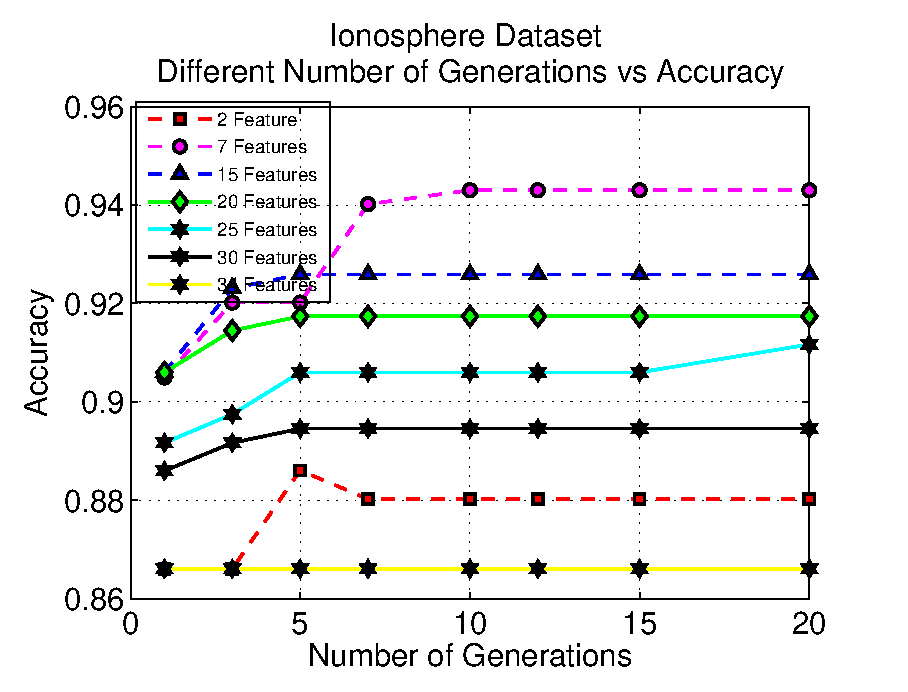
\includegraphics[width=0.45\linewidth]{img/ionfeat.eps}
      \label{fig:digraph}
    \end{figure}
Further testing performed was related to observe the behaviour of accuracy within the same number of features used but with varying the number of generations. In this experiment for the 2, 7, 15, 20, 25, 30, 35 numbers of features we varied the number of generation to 1, 3, 5, 7, 10, 15 and 20. For 1 feature taken, accuracy converges to 88\% after the 7th generation and remains identical till the 20th. For 7 features there is an increase between the 1st generations and the 5th from 90\% to 92.02\%. Also from the 7th generation onwards accuracy becomes stable acquiring the value of 94.3\%. For 15 features the same behaviour is observed with the accuracy increase from 1st generation till the 3rd from 90.6\% to 92.3\%. Above the 3rd generation the value remains the same. The same behaviour applies to the other number of features taken as shown in figure.
    \begin{figure}[h]
      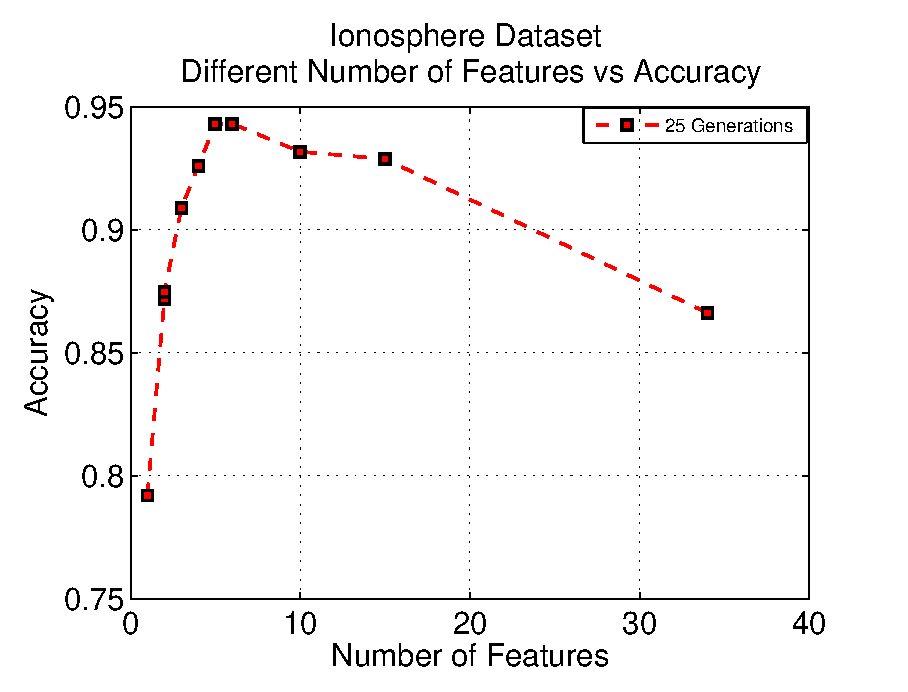
\includegraphics[width=0.45\linewidth]{img/ionfeat2.eps}
      \label{fig:digraph}
    \end{figure}


\subsection{Semeion Handwritten Digit Dataset }

    \begin{figure}[t]
      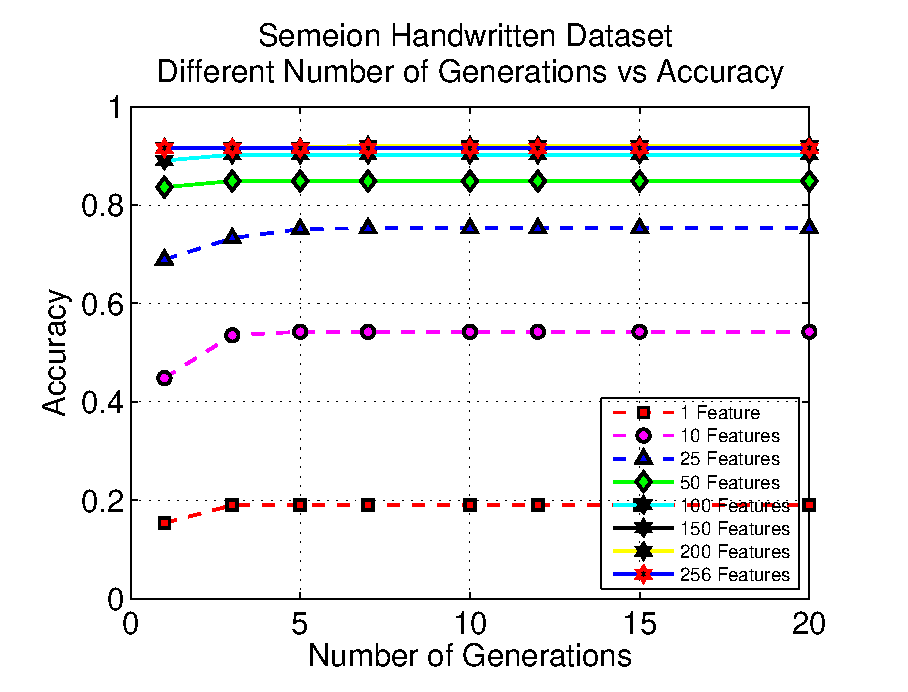
\includegraphics[width=0.45\linewidth]{img/seimfeat.eps}
      \label{fig:digraph}
    \end{figure}
     
    \begin{figure}[t]
      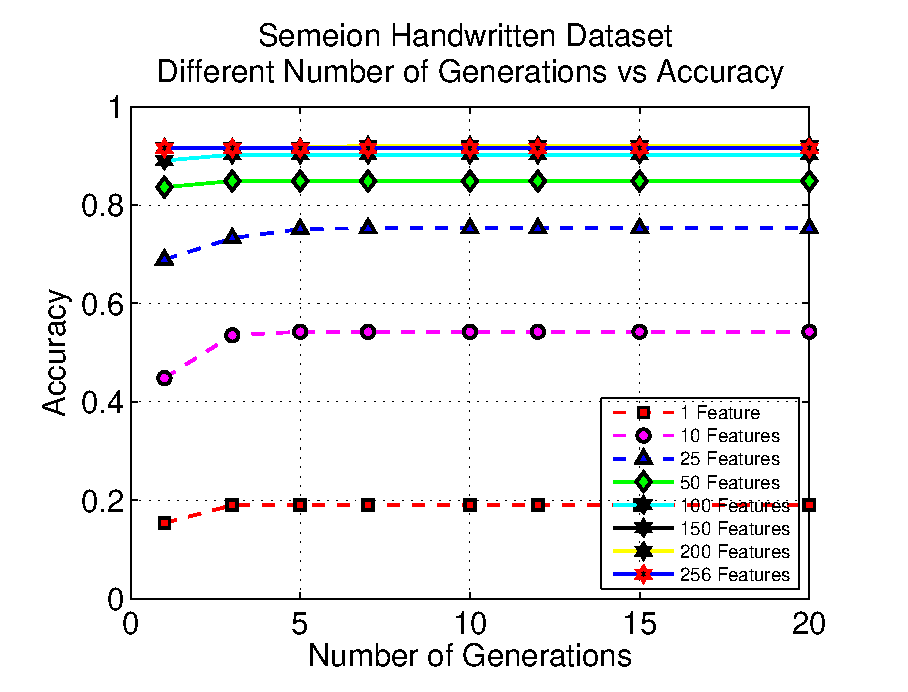
\includegraphics[width=0.45\linewidth]{img/seimfeat.eps}
      \label{fig:digraph}
    \end{figure}

\subsection{Red Wine Dataset }

   \begin{figure}[ht]
      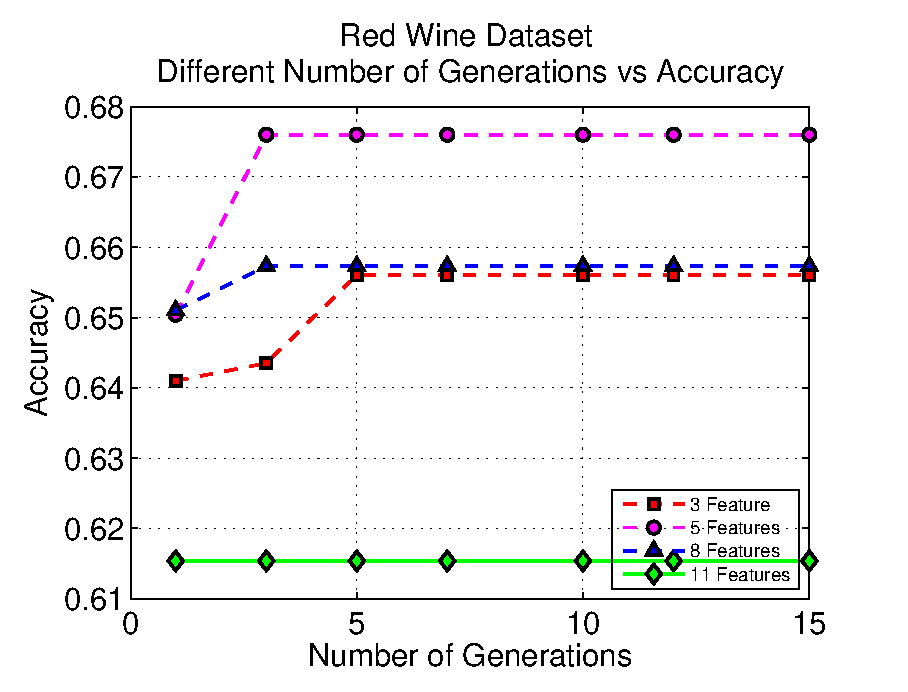
\includegraphics[width=0.45\linewidth]{img/winefeat.eps}
      \label{fig:digraph}
   \end{figure}

   \begin{figure}[ht]
     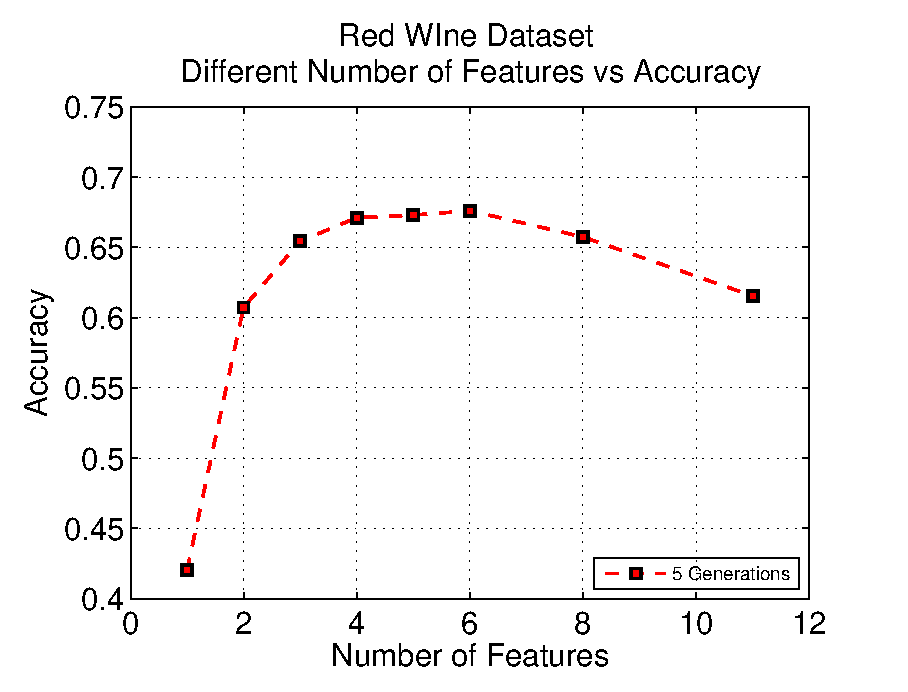
\includegraphics[width=0.45\linewidth]{img/winefeat2.eps}
     \label{fig:digraph}
   \end{figure}



\section{Conclusion}


{\small
\bibliographystyle{ieee}
\bibliography{egbib}
}

\end{document}
